\documentclass[a4paper,11pt]{article}
\usepackage[spanish]{babel}
\usepackage[utf8]{inputenc}
\usepackage{geometry}
\usepackage{booktabs}  
\usepackage{graphicx} 
\usepackage{listings}
\usepackage{amsmath,amsthm,amssymb}
\usepackage{float}

\lstset{%
backgroundcolor=\color{cyan!10},
basicstyle=\ttfamily,
numbers=left,numberstyle=\scriptsize
}

\setlength{\parskip}{\baselineskip}%
\setlength{\parindent}{0pt}%

%\usepackage[wby]{callouts}
\usepackage{hyperref}

\title{Memoria Proyecto Final}
\author{Álvaro Beltrán y Yábir García}
\begin{document}

\maketitle

\begin{figure}[h]

\includegraphics[scale=0.3]{UGR}
\centering
\end{figure}

\newpage

\renewcommand*\contentsname{Índice}
\tableofcontents

\newpage

\section{Definición del problema a resolver y enfoque elegido}

Para nuestro proyecto nos hemos decantado por trabajar con el conjunto de datos
\textit{Adult Census Income} recogido por Ronny Kohavi y Berry Becker. 

Se nos presenta un conjunto muestras para las que se han recogido distintos
parámetros que pueden afectar a la cantidad de dinero que se ingresa. Las
variables, las cuales se analizarán posteriormente, abarcan desde la ] edad
hasta el país de origen y el problema consiste en determinar cuando una muestra
va superar las 50000 unidades monetarias de ingresos y cuando se va a mantener
por debajo.

Estamos ante un problema de aprendizaje supervisado en el ámbito de la
clasificación binaria. En nuestro caso los elementos que intervienen en el
aprendizaje son 

\begin{itemize}
    \item $X$: Conjunto de datos relativos a una persona que pueden tener
    repercusión en el dinero que gane. Se trata de un vector que mezcla
    variables categóricas con variables reales.
    \item $y$: Es un valor en el conjunto $\{0,1\}$ que nos indica si los
    ingresos superan las 50000 unidades monetarias o no.
    \item $f$: Función que nos relaciona el conjunto $X$ con $y$ de manera que a
    cada muestra le asigna su categoria de ingresos.
\end{itemize}

En este problema es dicha función $f$ la que queremos aproximar. Para ello vamos
a basar nuestro estudio en aplicar el conocimiento adquirido durante la
asignatura utilizando métodos lineales y no lineales.

\section{Obtención de los datos}

Para la obtención de los datos hemos utilizado el repositorio público de
\textit{UCI}, más concretamente la url
\href{https://archive.ics.uci.edu/ml/machine-learning-databases/adult/}{https://archive.ics.uci.edu/ml/machine-learning-databases/adult/}.
Podemos apreciar como hay distintos archivos entre los que se encuentran los
datos y una descripción. 

Los datos aparecen separados en dos archivos distintos, uno para training y otro
para test. Descargamos ambos ficheros (\textit{adult.data}, \textit{adult.test})
y en nuestro trabajo hemos decidido combinarlos para realizar una separación
propia.

El motivo de esta elección es que como se verá a continuación hay un alto número
de muestras del total disponible a las que le falta el valor de alguna columna.
Como en general son unas columnas concretas en las que las muestras no estan
provistas del valor, se ha seguido el criterio expuesto en el guión de asignar
un valor aleatorio en función de una distribución multinomial. Es por esto que
hemos creido correcto que era mejor juntar los datos, aproximar los valores que
faltaban y crear conjuntos de test y training basados en una poporción 80-20
(80\% de los datos para training y 20\% para test).

\section{Argumentos a favor de la elección de los modelos.}

En cuanto a los modelos lineales elegidos nos hemos decantado por Regresión
Logística y Perceptron, debido a que son dos modelos que hemos estudiado en
clase para ejemplos de clasificación binaria, como es nuestro caso.  

Además parece interesante probar con el Perceptron puesto que también vamos a
usar el perceptron multicapa (MLP). Y puesto que Regresión Logística ha dado tan
buenos resultados en las prácticas de esta asignatura y suele funcionar muy bien
en clasificación parece indispensable probar este modelo.

De los modelos no lineales propuestos hemos elegido Perceptron Multicapa, Random
Forest y SVD.

Vamos a usar Ramdom Forest por que suele ser bueno para clasificación, a parte
de que es poco sensible a cambios en el conjunto de train (vamos a usar
validación cruzada). Además, de los algoritmos actuales ninguno le supera en
precisión y nuestros datos no están correlados factor que mejora su
rendimiento.

Perceptron Multicapa es un modelo que nos permite aprender funciones no lineales
utilizando la técnica de \textit{backpropagation}. Este tipo de algoritmos son
interesantes ya que nos permiten aprender relaciones entre las variables y cual
es la mejor manera con la que relacionarlas con nuestra función de salida. Es
por esto que esta técnica tiene gran interés y por lo que nosotros hemos
decidido usarala.

SVC. En nuestro caso nos hemos decantado por utilizar también un algoritmo de tipo
Suport Vector Machine preparado para hacer clasificación. Hemos visto que es una 
técnica muy potente que puede darnos muy buenos resultados cuando tenemos un alto 
número de características. Este a priori, no es nuestro caso pero cuando, como a 
continuación veremos, recodifiquemos las variables observaremos que el número 
de variables crecerá y esta técninca nos puede proporcionar resultados de interes.

\section{Exploración y preprocesado de los datos}

En primer lugar vamos a analizar el típo de variables con los que contamos. Este
análisis lo recogemos en la siguiente tabla

\begin{table}[h!]
    \centering
    \begin{tabular}{|c|c|c|}
    \hline
    Variable & Tipo de variable & Número de categorías\\ \hline
    age & continua & - \\ \hline
    workclass & categórica & 8 \\ \hline
    fnlwgt & continua & - \\ \hline
    education & categórica & 16 \\ \hline
    education-num & continua & - \\ \hline
    marital-status & categórica & 7 \\ \hline
    occupation & categórica & 14 \\ \hline
    relationship & categórica & 6 \\ \hline
    race & categórica & 5 \\ \hline
    sex & categórica & 2 \\ \hline
    capital-gain & continua & - \\ \hline
    capital-loss & continua & - \\ \hline
    hours-per-week & continua & - \\ \hline
    native-country & categórica & 41 \\ \hline
\end{tabular}
\caption{Variables estudiadas en las muestras, su tipo y la cantidad de categorías si procede.}
\end{table}

Respecto al total del conjunto de datos nos encontramos que disponemos de
48843 muestras contando las que tenemos en los ficheros \textit{adult.data}
y \text{adult.test}. 

De estas 48843 una es una irregularidad en el archivo \textit{adult.test} que contiene 
una linea no válida.

Los datos contienen 14 columnas que se corresponden a 13 características mas 
la etiqueta que se predice. De entre las muestras las características que mas datos
perdidos tienen son 

\begin{enumerate}
    \item occupation con 2810 valoers perdidos
    \item workclass con 2800 valores perdidos 
    \item native-country con 858 valores perdidos 
\end{enumerate}

el resto de características solo tienen un valor perdido que se corresponde 
con la linea erronea en el archivo de \textit{adult.test}.

En lo que respecta al número de clases aproximadamente un $75\%$ se corresponden 
con la etiqueta $<=50K$ y un $25\%$ con la etiqueta $>50K$ (etiquetas que hemos
codificado como $0$ y $1$ respectivamente). En el siguiente gráfico se puede apreciar 
dicha diferencia en el número de muestras de cada clase 

\begin{figure}[h!]
    \centering
    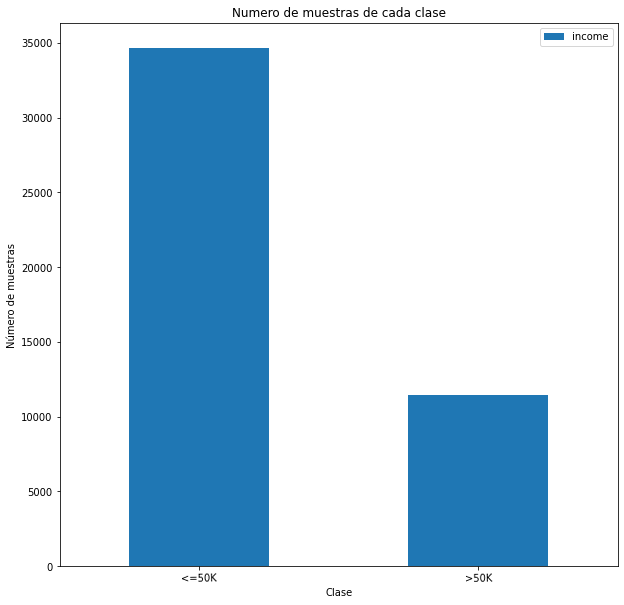
\includegraphics[width=0.7\textwidth]{images/proportion}
    \caption{Proporcion de muestras en cada clase}
\end{figure}


\subsection{Codificación de las variables}

Tenemos un conjunto de variables en las que se combinan tipos continuos y
categóricos por lo que nos va a resultar necesario convertir los datos
categóricos a valores reales. Para ello hemos optado por realizar para cada
variable de tipo categórico un vector de ceros y unos que representa con un uno
la pertenencia a una categoría concreta. Por ejemeplo en el caso de la variable
\textit{sex} que cuenta con dos categorías, $(1,0)$ representaría la pertenencia
al sexo femenino y $(0,1)$ al sexo masculino. En esta codificación de los datos
no es posible obtener un vector con más de un uno ya que en nuestros datos no se
pertenece a dos categorías de manera simultanea.

En nuestro caso nos hemos decantado por utilizar el método de pandas
\textit{get\_dummies}, que nos proporciona este comportamiento incluyendo la
codificación como variables en nuestro \textit{dataframe} de trabajo.

\subsection{Valoración del interes de las variables y selección de un subconjunto}

En principio, tras leer la descripción de los atributos estudiados. Solo vemos
dos variables que no aportan información al problema. La primera es
\textit{Education-num} que es una representación numérica del atributo education, no
aporta nada pues hemos tomado la decisión de dividir cada variable categórica en
una serie de variables donde asignamos 1 si es de un determinado tipo del
dominio de la variable o 0 si no es de ese tipo. La segunda variable es "fnlwgt"
que determina el número de personas representadas con esa instancia, entendemos
que esa variable no aporta información de fuera de la muestra y por lo tanto no
es interesante.

\subsection{Normalización de las variables}

Los rangos en los que se mueven las variables son muy dispares y normalmente con
valores muy distantes por lo que hemos visto conveniente realizar una
normalización de las variables continuas. Para ello hemos aplicado
\textit{StandardScaler} de sklearn de manera que transforma la variables
dejandolas con medio 0 y varianza 1. De esta forma  todas las variables se
encuentran centradas entorno al mismo valor y en un rango similar. 

Esto es un paso muy importante ya que afecta directamente al funcionamiento 
de los algoritmos que se van a desarrollar.

\subsection{Valores perdidos}

En cuanto a los valores perdidos hemos seguido las directrices propuestas en el
enunciado, hemos eliminado las instancias cuyos valores perdidos superaran el
10$\%$ (2 atributos con valores perdidos). Una vez eliminadas estas instancias
hemos rellenado los valores perdidos restantes con la multinomial asignando a
cada posible valor del domino del atributo una probabilidad dependiendo de la
cantidad de veces que aparecen en las instancias. Para ello, hemos usado la
funcion choice de la libreria random, determinando el dominio y las
probabilidades con las que aparecen cada objeto del dominio.


\section{Regularización}

En el caso del modelo lineal nos hemos decantado por utilizar regularización
basada en la norma 1, \textit{l1}, ya que hemos encontrado que no existe una
alta correlación lineal entre las variables y, con la introducción de las
variables \textit{dummies}, creemos que es la mejor elección. 

Para el algoritmo de random forest no se utiliza de manera implicita ningún
factor de regularización.

En el caso de SVC, el único parámetro que se puede moficiar es el coeficiente de
regularización, para el cual se ha aplicado un criterio de búsqueda en la
elección de hiperparámetros, pero no se puede elegir la métrica con la que se
regulariza.


\section{Justificación de la función de pérdida usada.}

En un principio pensamos en usar exactitud (Accuracy), pero esta métrica no
funciona bien cuando las clases están desbalanceadas como es en este caso. Así
que, es muy fácil acertar diciendo que dicha predicción está en la clase más
probable. Para problemas con clases desbalanceadas es mucho mejor usar
precisión. Esta métrica da una mejor idea de la calidad del modelo. 
\begin{align*}
\frac{TP}{TP+FP}
\end{align*}


Si llamamos la clase negativa a la clase mayoritaria, recibir menos de 50K u.m y
positiva a la clase minoritaria, recibir mas de 50K u.m. Con la métrica
(\textit{precission}) \cite{metrics} nos concentramos mas en la clase positiva y
en la probabilidad de de detectar la clase positiva y no tanto en distinguir la
clase negativa de la positiva.

Esta métrica era nuestra primera idea pero, al no plantearse contexto en el problema,
no existe un criterio que nos haga centrarnos en una clase respecto a otra. Por este 
motivo hemos considerado que la mejor opción era utilizar la métrica $F_1$ 
que se define como 

\[
    F_1 = 2\frac{\text{Precission} * \text{Recall}}{\text{Precission} + \text{Recall}} 
\]

donde \textit{Recall} es la métrica que nos da 

\[
    \frac{TP}{TP+FN}
\]

Usando $F_1$ como métrica lo que hacemos es tener un equilibrio entre Recall y
Precission con lo que no favorecemos ningún comportamiento y entrenamos de una manera 
más general.

\section{Estimación de los hiperparámetros.}

%rellenar hiperparametros de los otros dos

Para los modelos estudiados anteriormente hemos seleccionado una serie de
parámetros y vamos a hacer inferencia sobre otros:

\begin{itemize}

\item \textbf{Regresión Logística}. Hemos decidido usar el solver lbfgs que es
newton pero con mejoras en memoria para reducir el tiempo, vamos a usar este
porque newton adapta la tasa de aprendizaje según le convenga y por tanto es más
eficaz. Usamos penalización L1 ya que usamos Lasso. Y hacemos inferencia sobre
los parámetros C y tol. El parámetro C es el coeficiente que acompaña a la
penalización y tol es la tolerancia usada en el modelo.

\item \textbf{Perceptron}. Hemos prefijado la máximas iteraciones a 2000 por que
probando con menos no acababa y hemos decidido que baraje los datos en cada
iteración del perceptron como hemos visto en teoría. Hacemos inferencia sobre
los parámetros alpha y tol. El parámetro alpha es el coeficiente que acompaña a
la penalización (elegida la que viene por defecto) y tol es la tolerancia usada
en el modelo.

\item \textbf{Ramdom Forest}. Vamos a usar bootstrap porque es capaz de medir la
incertidumbre de nuestro modelo mediante una técnica de reelección de muestras.
Para determinar las máximas características del árbol vamos a usar la raíz
cuadrada por que hay evidencias empíricas de que es el mejor. Hemos hecho
inferencia sobre el criterio de selección, sobre si elegir entropy o gini. 

\item \textbf{MLPClasiffier} (Perceptron Multicapa).Hemos decidido usar el
solver lbfgs que es newton pero con mejoras en memoria para reducir el tiempo,
al igual que hicimos en Regresión Logística. También hemos fijado las
iteraciones máximas a 20000 por que si no, no conseguía converger. Además,
hacemos inferencia sobre los parámetros alpha (ya explicado antes) y función de
activación. Para la función de activación damos tres opciones, 'logistic',
'tanh', 'relu': $ \frac{1}{1 + exp(-x)} , tanh(x), max(0, x)$ respectivamente.

\item \textbf{SVC}. Para este modelo hemos fijado los parámetros kernel y gamma
a rbf y scale respectivamente. Elegimos rbf por que es un kernel no lineal que
no añade demasiada complejidad y \textbf{ scale por que }. Y hacemos inferencia
sobre el parámetro C que ya hemos explicado en Regresión logística.

\end{itemize}

\section{Resultados obtenidos}

\subsection{Regresión Logística}

En el caso de la regresión logistica los mejores parámetros que se han obtenido 
han sido:

\begin{itemize}
    \item Coeficiente de regularización: $1000000.0$
    \item Penalty: $l2$
    \item Solver: \textit{lbfgs}
    \item Tolerance: $0.001$
\end{itemize}

Los resultados que se han obtenido han sido los siguientes:

\begin{table}[h!]
\centering
\begin{tabular}{|l|l|l|}
\hline
Algoritmo    & $E_in$  & $E_{out}$ \\ \hline
 Regresión Logística   & 71.9281 & 71.0873 \\ \hline
\end{tabular}
\caption{Resultados para regresión logistica con los mejores parámetros}
\end{table}

\subsection{Perceptron}

\begin{itemize}
    \item Coeficiente alpha: $1.0$
    \item max\_iter: $2000$
    \item Shuffle: $True$
    \item Solver: \textit{lbfgs}
    \item Tolerance: $0.0031622776601683794$
\end{itemize}

Los resultados que se han obtenido han sido los siguientes:

\begin{table}[h!]
\centering
\begin{tabular}{|l|l|l|}
\hline
Algoritmo    & $E_in$  & $E_{out}$ \\ \hline
Perceptron & 53.8586 & 53.4161 \\ \hline
\end{tabular}
\caption{Resultados para perceptron con los mejores parámetros }
\end{table}

\subsection{Random Forest}

\begin{itemize}
    \item Bootstrap: \textit{True}
    \item Criterio: \textit{gini}
    \item max\_fatures: \textit{sqrt}
    \item min\_samples\_split: $5$
\end{itemize}

Los resultados que se han obtenido han sido los siguientes:

\begin{table}[h!]
\centering
\begin{tabular}{|l|l|l|}
\hline
Algoritmo    & $E_in$  & $E_{out}$ \\ \hline
Random Forest   & 89.9642 & 70.9722 \\ \hline
\end{tabular}
\caption{Resultados para random forest con los mejores parámetros}
\end{table}

\subsection{Multilayer Perceptron}

\begin{itemize}
    \item Activation: \textit{logistic}
    \item Alpha: \textit{5}
    \item max\_fun: 20000
    \item solver: \textit{lbfgs}
\end{itemize}

\begin{table}[h!]
    \centering
    \begin{tabular}{|l|l|l|}
    \hline
    Algoritmo    & $E_in$  & $E_{out}$ \\ \hline
    MLP   & 73.8746 & 73.0701 \\ \hline
    \end{tabular}
    \caption{Resultados para MLP con los mejores parámetros}
\end{table}

\subsection{Recopilación de los resultados}

Procedemos a recuperar los resultados en una única tabla

\begin{table}[H]
    \centering
    \begin{tabular}{|l|l|l|}
    \hline
    Algoritmo    & $E_in$  & $E_{out}$ \\ \hline
    Regresión Logística   & 71.9281 & 71.0873 \\ \hline
    Perceptron & 53.8586 & 53.4161 \\ \hline
    Random Forest   & 89.9642 & 70.9722 \\ \hline
    MLP   & 73.8746 & 73.0701 \\ \hline
    \end{tabular}
    \caption{Resultados con los mejores parámetros}
\end{table}

\section{Elección del mejor modelo}

Tras haber realizado una elección de los mejores parámetros de cada modelo hemos 
decidido volver a aplicar la técnica de validación cruzada 

\section{Conclusiones}

Aquí decir que lineal good y que no hay nada que envidiar

%comparación entre modelos lineales y no lineales
%los resultados 
%las gráficas 
%confusion matrix
%ideonidad de los modelos


%cosas que no se rellenar: porque gamma=scale, porque hemos decidido usar MLP y SVC
%revisar métrica


\end{document}
